\documentclass[utf8,aspectratio=43]{beamer}
\usepackage[french]{babel}
\usepackage[T1]{fontenc}

\usepackage{amsmath, amsfonts, graphicx}
\usepackage{bibunits, tikz}
\usepackage{stmaryrd}

\usetheme{progressbar}
\graphicspath{{images/}}

\setbeameroption{show notes}
\setbeamersize{text margin left=1em, text margin right=1em}

%\begin{itemize}
%	\item Brought to you by Cédric Mauclair
%	\item Please let me know about improvements!
%	\item Inspiration: \url{http://www.shawnlankton.com}... (in code)
%\end{itemize}

\title[
Optimisation de trajectoire et du temps de mission d'un drone de
télécommunication multicast.
]{
  Trajectory Optimization for Completion Time Minimization in
  UAV-Enabled Multicasting
}

\author[Hondet, Viry, Beldjilali]{
  G.~Hondet\quad B.~Viry\quad A.~Beldjilali}

\date{12 Décembre 2018}

\institute{ENAC}

\begin{document}


\maketitle

\begin{frame}{Plan}
\tableofcontents
\end{frame}


	
	\maketitle

\section {Introduction}

\begin{frame}{Introduction}
  L'article présente une optimisation de trajectoire d'un drone qui doit transmettre, i.e. disséminer, i.e multicaster,
  en un minimum de temps un même fichier à des récepteurs terrestres via une communication sans fil.
\end{frame}

\begin{frame}{Plan}

\tableofcontents

\end{frame}
%\section{Modélisation du système et du problème}

\subsection[Modèle initial]{Formulation et modélisation initiale du problème}
\begin{frame}{Formulation initiale}
  \begin{itemize}
  \item Minimiser le temps d'exécution de la mission
  \item sous contraintes
    \begin{itemize}
    \item \( \forall k \in \mathcal{K}, P_{k, \text{succ}} \geq
      \bar{P} \),
          \note[item]{\( \mathcal{K} \) ensemble des terminaux }
    \item vitesse max de l'UAV \( V_{\text{max}} \)
    \end{itemize}
  \end{itemize}
      
\end{frame}



\begin{frame}{Modélisation temps et position}
  \begin{block}{Discrétisation}
    \[ T = M \delta_t \]
    \note[item]{\( T \) horizon de la mission}
    \note[item]{\( M \) pas de temps final}
    \note[item]{\( \delta_t \) durée d'un pas de temps}
    \begin{equation}
      \min \text{\textit{temps d'exécution de la mission}}
      \longleftrightarrow \min_M M
    \end{equation}
  \end{block}
  \begin{block}{Position et vitesse}
    \begin{itemize}
    \item Position \( \mathbf{q}[m]_{m = 1}^M \in \mathbb{R}^{2 \times
      M} \)
    \item Déplacement maximal \( \tilde{V}_{\text{max}} = \delta_t
      V_{\text{max}} \)
    \end{itemize}
    \begin{equation}
      \text{\textit{UAV restreint à}} V_{\text{max}} \longleftrightarrow
      \forall m, \| q[m] - q[m - 1] \| \leq \tilde{V}_{\text{max}}
    \end{equation}
  \end{block}
\end{frame}
\begin{frame}{Réception des paquets}
  \begin{itemize}
  \item \( N_k \) nombre de paquets reçus par terminal \( k \)
  \item \( N' \) nombre de paquets nécessaire
  \item \( N \) nombre de paquets codés transmis
    \note[item]{\( N \) donné par RLNC}
  \end{itemize}
  \begin{block}{Qualité de transmission}
    \begin{equation}
      \text{\textit{probabilité de réception correcte}} \longleftrightarrow
      \mathbb{P}(N_k \geq N')
    \end{equation}
    \note[item]{
      avec \( N_k \sim \mathcal{P} \) vu que \( N_k = \sum_{m = 1}^M
      \sum_{l = 1}^L Z_k[m, l] \) avec \( Z_k[m, l] \) suivant une loi de
      Bernouilli indiquant si terminal \( k \) a reçu le paquet \( l \) du
      time slot \( m \)
    }
  \end{block}
\end{frame}
\begin{frame}{Modélisation initiale}
  \begin{align}
      & \min_{q[m]_{m=1}^M, M} M \tag{P1} \label{eq:init-obj} \\
      \text{s.t. } & \forall k \in \mathcal{K}, P_{k, \text{succ}}
      \geq \bar{P} \label{eq:init-prec} \\
      & \forall m \in \llbracket 1, M \rrbracket, \| q[m] - q[m - 1]
      \| \leq \tilde{V}_{\text{max}}
  \end{align}
\end{frame}

\subsection{Minoration de la probabilité de succès}
\begin{frame}{Minoration de \( P_{k, \text{succ}} \)}
  \begin{alertblock}{Problème}
    \( P_{k, \text{succ}} \) dépend de \( \mathbf{q} \)
    \note[item]{probabilité de réception diminue quand la distance
      augmente}
  \end{alertblock}
  \begin{block}{Distance caractéristique}
    On introduit \( D \) tel que
    \[ \| \mathbf{q}[m] - \mathbf{w}_{k} \| > D \implies
      \text{réception impossible} \]
  \end{block}
\end{frame}
\begin{frame}{Minoration}
  \( \mathcal{M}_{k, D} = \{ m | \| \mathbf{q}[m] - \mathbf{w}_k \|
  \leq D \} \)
  \note[item]{\( \mathcal{M}_{k, D} \) ensemble des pas de temps
    durant lesquels la transmission est réalisable}
  \begin{block}{Minorant}
    \( \hat{N}_k \) un minorant du nombre de paquets reçus par
    terminal \( k \)
    \note[item]{\( \hat{N}_k \sim \mathcal{B}(| \mathcal{M}_{k, D} |
      L, p_D)\)}
    \note[item]{\( L \) nombre de paquets transmis par time slot}
    \note[item]{\( p_D \) proba de réception d'un paquet à distance \(
    D \)}
    \begin{equation}
      P_{k, \text{lb}} = \mathbb{P}(\hat{N}_k \geq N')
    \end{equation}
  \end{block}
\end{frame}

\subsection{De la probabilité au temps}
\begin{frame}{De la probabilité au temps}
  \begin{block}{Approximation}
    \[ \hat{N}_k \approx \mathcal{G}(\mu, \sigma^2) \]
    \( \mu, \sigma^2 \) dépendant de \( | \mathcal{M}_{k, D} |, L, p_D
    \)
  \end{block}
  \begin{equation}
    P_{k, \text{lb}} = \mathbb{P}(\hat{N}_k \geq N) \approx
    Q\left(f(N', | \mathcal{M}_{k, D} |, L, p_D) \right)
  \end{equation}
  \note[item]{\( Q \colon x \mapsto \int_x^{\infty} e^{-u^2 / 2} \,
    \mathrm{d}u \)}
  \note[item]{\( f \) est une fonction connue}
  \begin{block}{Expression en temps}
    \begin{equation}\label{eq:1}
      | \mathcal{M}_{k, D} | \geq M_{\text{min}}
    \end{equation}
    \( M_{\text{min}} \) connu dépendant de \( L, p_D, N' \) et \(
    Q^{-1}(\bar{P}) \)
  \end{block}
\end{frame}
\begin{frame}{C'est bientôt la fin}
  \begin{align}
    \label{eq:2}
    & \min_{q[m]_{m=1}^M, M} T = \delta_t M \tag{P3} \\
    \text{s.t. } & \forall k \in \mathcal{K},
                   | \mathcal{M}_{k, D} | \geq M_{\text{min}} \\
    & \forall m \in \llbracket 2, M \rrbracket,
      \| q[m] - q[m - 1] \| \leq \tilde{V}_{\text{max}}
  \end{align}
\end{frame}

\subsection{Trajectoire explicitée}
\begin{frame}{Re modélisation de la trajectoire}
  \begin{block}{Relaxation du TSP}
    Regroupement des terminaux en \( \mathcal{S}_g \)
    \note[item]{\( \mathcal{S}_g \) zone de rayon \( D \) regroupant
      plusieurs terminaux}
    \note[item]{Zones \( \mathcal{S}_{g} \) données par un algo non
      exposé ici}
    \note[item]{Pour couvrir tous les terminaux de la zone \(
      \mathcal{S}_g \), il suffit de passer dans la zone}
  \end{block}
  \begin{align}
    & \min_{
        {\{\mathbf{s}_g, \mathbf{f}_g\}}_{g=1}^G
      }
      \underbrace{
      \sum_{g = 1}^G \max \left\{
      \frac{
      \| \mathbf{f}_g - \mathbf{s}_g \|
      }{
      V_{\text{max}}
      }, T_{\text{min}}
      \right\}
      }_{\text{traversée}} +
      \underbrace{
      \sum_{g = 1}^G
      \frac{
      \| \mathbf{s}_{g + 1} - \mathbf{f}_g \|
      }{
      V_{\text{max}}
      }
      }_{\text{transition}} \tag{P4} \\
    \text{s.t. } & \forall g, (\mathbf{s}_g, \mathbf{f}_g) \in \mathcal{C}_g
  \end{align}
\end{frame}

\subsection{Optimisation de la vitesse}
\begin{frame}{Optimisation de la vitesse}
  \begin{block}{Variable de décision}
    \begin{itemize}
    \item Discrétisation en espace, \( \delta_t \rightsquigarrow
      \delta_d \)
    \item Manipulation du temps, \( \mathbf{q}[m] \rightsquigarrow
      \tau_j \)
    \end{itemize}
  \end{block}
  \begin{align}
    & \min_{\{\tau_j\}_{j = 1}^J} \sum_{j = 1}^J \tau_j \tag{P5} \\
    \text{s.t. } & \forall k \in \mathcal{K}, \sum_{j = 1}^J I_{kj}
                   \tau_j \geq T_{\text{min}} \\
    & \forall j \in \llbracket 1, J \rrbracket,
      \tau_j \geq \frac{\delta_d}{V_{\text{max}}}
  \end{align}
  \note[item]{Discrétisation en espace donne \( \{\mathbf{q}_j\}_{j =
  1}^J \) ensemble de positions à chaque pas de déplacement}
  \note[item]{Avec \( I_{kj} = 1 \) si UAV en connexion avec terminal
    \( k \) quand en \( j \)\textsuperscript{ième} position}
\end{frame}
%%% Local Variables:
%%% mode: latex
%%% TeX-master: "atp"
%%% End:

%\section{Reformulation du problème}
\subsection{Borne inférieure de la probabilité de bonne réception $P_{k,succ}$}
\begin{frame}{Borne inférieure de la probabilité de bonne réception $P_{k,succ}$}
Borne inférieure de la probabilité
 
\end{frame}


\subsection{Le problème reformulé}
\begin{frame}{Le problème reformulé}

problème simplifié
\end{frame}

%
% Equations are easy
%\begin{itemize}
%	\item Just copy/paste equations\pause
%	\item From the paper!
%	\begin{equation*}
%	\textbf{p}^* = \underset{\textbf{p}}{\arg\!\min}~\sum_{\textbf{x}}\left[ I(\textbf{W}(\textbf{x};\textbf{p})) - T(\textbf{x}) \right]^2
%	\end{equation*}
%\end{itemize}
%\end{frame}
%% % % % % % % % % % % % % % % % % % % % % % % % % % % % % % % % % % % % % % % % % % % % % % % % % 
\section{Résultats}

\subsection{Conception des waypoints}
\begin{frame}{Conception des waypoints}
conception de la trajectoire
\end{frame}

\subsection{Optimisation de la vitesse du drone}

\begin{frame}{Optimisation de la vitesse du drone}
vitesse drone optimisation
\end{frame}
% % % % % % % % % % % % % % % % % % % % % % % % % % % % % % % % % % % % % % % % % % % % % % % %

\section{Conclusion}


\begin{frame} {Résumé}

Cet article a donc présenté 
\begin{itemize}
	\item un cas d'optimisation de trajectoire 4D
	\item contraint par la vitesse maximale du drone
	\item et par le temps minimum de connexion nécessaire à bonne réception du message. 
\end{itemize}


\end{frame}


% % % % % % % % % % % % % % % % % % %ù

\begin{frame} {}

Pour ce faire, plusieurs étapes ont été nécessaires

\begin{enumerate}
	\item Reformulation du problème en utilisant une seule contrainte
	de temps minimum de connexion entre le drone et le terminal terrestre.\pause
	
	\item Les auteurs ont ensuite montré que la trajectoire optimale
	peut-être constituée uniquement de segments de droites reliant des
	waypoints dont la position est optimisée.\pause
	\item Ils ont calculé la position optimale de ces waypoints.
	Ce qui définit une trajectoire optimale. \pause 
	\asuivre
	
\end{enumerate}
\end{frame}	
	
\begin{frame} {Résumé}



\begin{enumerate}	
	
	 \suite
	\item Puis ils optimisent la vitesse en fonction du temps le long de la trajectoire obtenue
	en utilisant la programmation linéaire(LP).\pause
	\item Les résultats numériques ont mis en évidence des performances significativement améliorées
	 par rapport à une approche heuristique de conception de trajectoires ou un système multicast statique.\pause
	\item Ce qui tend à montrer le grand potentiel des drones de 
	télécommunication à usage de transmetteurs multicast dans les réseaux sans-fil.
	 
\end{enumerate}
\end{frame}



\begin{frame} {Critiques}
\begin{itemize}
	\item Article bien écrit qui couvre un spectre de connaissances assez large : telecom, stat, RO, optimisation.
	\item Article assez difficile car couvre divers domaines : Télécom., Recherche Opérationnelles, Statistiques
	\item Plan annoncé, suivi et rappelé dans la conclusion
	\item Notations bien explicitées
	\item Bibliographie pertinente
	\item Il manquerait une application concrète, in situ, des résultats obtenus.
	\item La notation F est trompeuse. Dans l'article, elle représente la complémentaire de la fonction de répartition, cette dernière étant généralement notée $\tilde{F}$.
\end{itemize}


\end{frame}



\begin{frame} {Perspectives}

\begin{enumerate}
	\item Phase multicast de transmission de paquets
	\item Phase device to device (D2D) : les terminaux s'échangent des paquets pour reconstituer le message dans leur totalité. 

\end{enumerate}



% \begin{figure}[t]
%	\centering
%	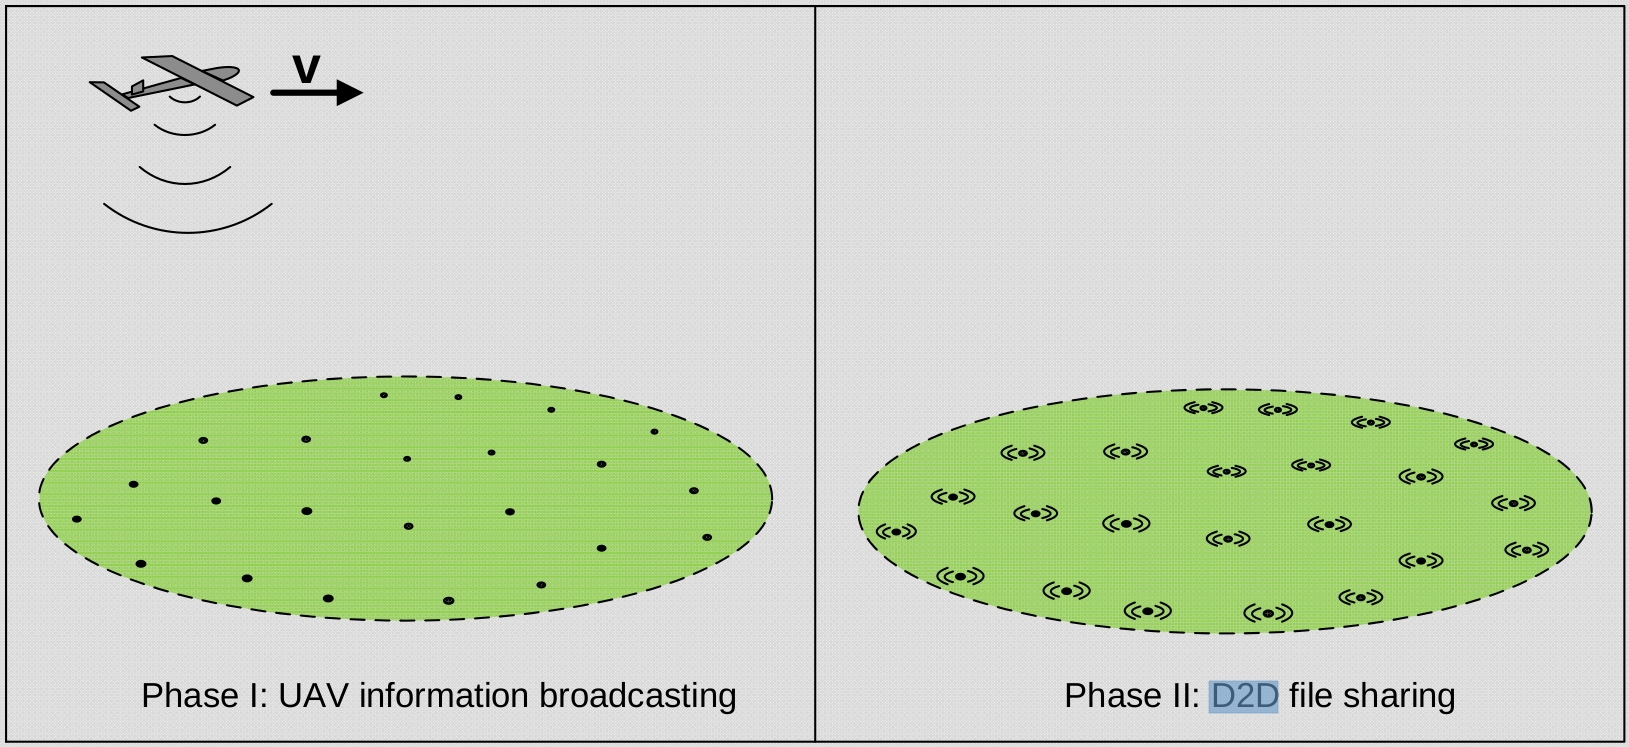
\includegraphics[height=\dimexpr11\textheight/16\relax]{d2d}
%	\caption{D2D}
%\end{figure}

\begin{figure}
	\centering
	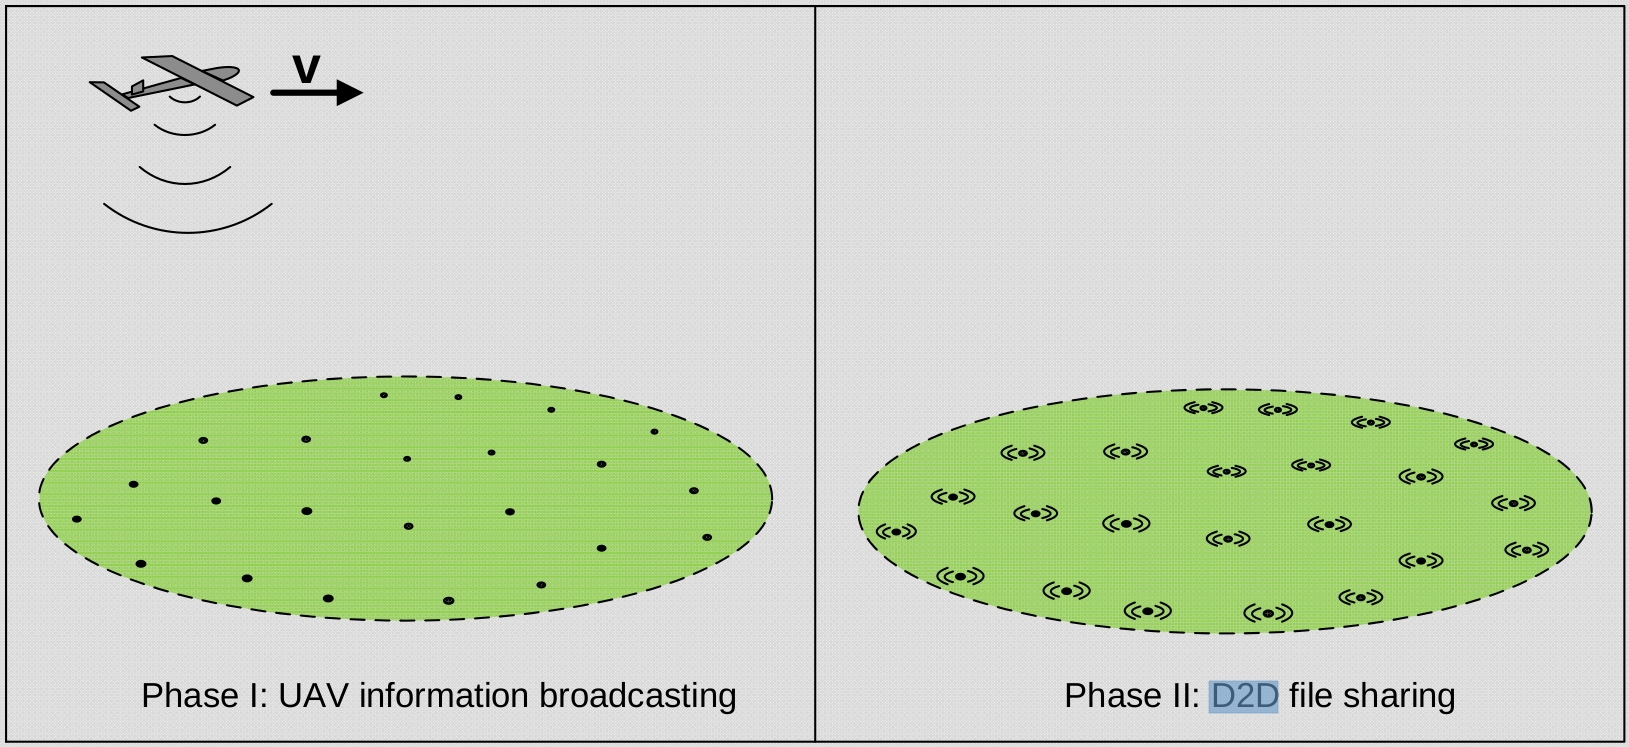
\includegraphics[width=1\linewidth]{d2d}
%	\caption{}
	\label{fig:d2d}
\end{figure}


\end{frame}


%\begin{frame} {}
%
%Cet article n'a pris en compte que la phase multicast. L'étude conjointe
%des deux phases multicast et D2D serait probablement intéressante à entreprendre.
%En lien avec des techniques de clustering pour les stations sol, l'optimisation
%conjointe pourrait permettre de réduire davantage les coûts de transmission et donc la taille des drones
%utilisés.
%
%\end{frame}



\end{document}


%\begin{block} {Some block}
%	
%	\begin{itemize}
%		\item Movies only seem to work in Adobe Reader
%		\item Movie file is not embedded, it must be on the computer
%	\end{itemize}
%\end{block}
%
%\pause
%\begin{alertblock}
%	{Some more block}
%	
%	Movies only seem to work in Adobe Reader\\
%	Movie file is not embedded, it must be on the computer
%\end{alertblock}
%\pause
%
%\begin{exampleblock}{}
%	Some text in here.
%	
%	\begin{itemize}[<+->]
%		\item Movies only seem to work in Adobe Reader
%		\item Movie file is not embedded, it must be on the computer and
%		what happe with a very long item?
%	\end{itemize}
%\end{exampleblock}
%

%\appendix[Appendices]
%
%\begin{frame}
%  \frametitle{First appendix}
%\end{frame}
%
%\begin{frame}
%  \frametitle{Second appendix}
%\end{frame}

% Things in a Bulleted List\pause
%
%\begin{enumerate}
%	\item Bullets that
%	\begin{enumerate}
%		\item one
%		\item two
%	\end{enumerate}\pause
%	\item Come up
%	\begin{enumerate}
%		\item one
%		\item \emph{two} and three
%	\end{enumerate}\pause
%	\item One by one
%	\begin{enumerate}
%		\item one
%		\item two
%	\end{enumerate}
%\end{enumerate}
